
A major experimental program is underway which seeks to measure
as of yet unknown properties associated with the change of flavor of neutrinos.
In particular, the neutrino mass hierarchy and charge-parity (CP) violating phase
of neutrinos still remain to be measured, with additional focuses on measuring
oscillation parameters with high precision and testing whether the current
three-flavor mixing paradigm is sufficient~\cite{Esteban:2020cvm, ParticleDataGroup:2020ssz}.
These goals introduce stringent requirements on the precision of current and future experiments.
High-intensity beams are required to produce the flux of neutrinos
 to be able to accumulate the necessary statistics.
Increased statistics place additional burden on the systematic uncertainties needed for the experimental program.

Two, billion dollar scale, next-generation experiments designed to meet these experimental constraints
are the Deep Underground Neutrino Experiment (DUNE)~\cite{Abi:2020wmh}
 and the Hyper-Kamiokande experiment (Hyper-K)~\cite{Hyper-Kamiokande:2018ofw}.
DUNE has a broad neutrino energy spectrum with a peak at a neutrino energy of $\approx$2.5 GeV,
but significant contributions between 0.1--10 GeV, over a 1295 km baseline. Hyper-K has a narrow
neutrino energy spectrum peaked at a neutrino energy of $\approx$0.6 GeV, with significant
contributions between 0.1--2 GeV, over a 295 km baseline. Despite their different energies and
baselines, both experiments sit at a similar L/E, so probe similar oscillation physics.
At the few-GeV energies of interest, neutrino interactions with nucleons have many available interaction channels,
 including quasielastic, resonant, and deep inelastic scattering~\cite{zeller12, hayato_review_2014, Mosel:2016cwa, Katori:2016yel, NuSTEC:2017hzk}.
All current and planned experiments use nuclear targets ($^{12}$C--$^{40}$Ar) as the
target material to increase the interaction rate, as well as to avoid serious experimental complications using elementary targets.
The use of nuclear targets significantly complicates the cross-section modeling issues and
associated systematics as intra-nuclear dynamics have a comparable energy scale to
the energy transfers in the neutrino interactions of interest.

A significant challenge impeding progress towards a consistent theoretical description of neutrino-nucleus interactions is the lack of data to benchmark parts of the calculation against. For example, neutrino quasielastic scattering ($\nu_{l} + n \rightarrow l^{-} + p$ or $\bar{\nu}_{l} + p \rightarrow l^{+} + n$) is the simplest of the relevant hard scattering processes, and dominates the neutrino cross section below $\approx$1 GeV. However, modern experiments using nuclear targets are unable to measure it without significant nuclear effects~\cite{garvey_review_2014, NuSTEC:2017hzk}.
Neutrino cross-section models for quasielastic scattering (and other hard-scattering processes) have relied heavily on sparse data from the 1960--1980's from several bubble chamber experiments which used $H_{2}$ or $D_2$ targets~\cite{zeller12, ParticleDataGroup:2020ssz}.
The small neutrino cross section, and relatively weak (by modern standards) accelerator neutrino beams utilized by these early experiments, mean that the available quasielastic event sample on light targets amounts to a few thousand events~\cite{ANL_Barish_1977, BNL_Baker_1981}.
{\color{red} [We could consider adding some comments about pion electroproduction here]}

The sparse data from deuterium bubble chamber experiments do not constrain
 the axial form factor precisely.
The popular dipole axial form factor ansatz has a shape that
 is overconstrained by data, which results in an underestimated uncertainty.
Employing a model-independent $z$ expansion parameterization
 relaxes the strict shape requirements of the dipole and yields
 a more realistic uncertainty that is nearly an order of magnitude larger.
The axial radius, which is proportional to the slope of the form factor at $Q^2=0$,
 has a 50\% uncertainty when estimated from the $z$ expansion.
Ideally, the lack of precision in the axial form factor would
 be rectified by a modern neutrino scattering experiment.

Safety considerations make it unlikely that new high-statistics bubble chamber experiments with
 hydrogen or deuterium fills will be deployed to fill this crucial gap,
 so experiments are looking for other ways to access neutrino interactions
 with elementary targets, as a tool for disambiguating neutrino cross section modeling uncertainties.
One possibility is to use experiments with various hydrocarbon targets to subtract the carbon interaction contributions from
 the total hydrocarbon event rates, and produce ``on hydrogen'' measurements~\cite{PhysRevD.92.051302, PhysRevD.101.092003, Hamacher-Baumann:2020ogq, DUNE:2021tad}.
 These ideas are promising, but typically rely on kinematic tricks that are only relevant for some channels, and it remains to be seen whether the model systematics associated with the carbon subtraction can be adequately controlled. Such ideas may also be extended to other compound target materials with hydrogen or deuterium components.

In the absence of an updated scattering experiment on an elementary target,
 lattice QCD (LQCD) could provide the missing free nucleon amplitudes
 that are otherwise not known at the required precision.
The nucleon axial form factor is the first benchmark quantity that could be computed,
 with a few-${\rm GeV}^2$ reach in momentum transfer possible.
A tension in the neutron magnetic form factor parameterization,
 which is roughly half the size of the total axial form factor uncertainty,
 could be resolved with a similar LQCD calculation.
More challenging computations could provide information about nucleon
 resonant and nonresonant contributions to axial matrix elements,
 such as the $\Delta$ or Roper resonance channels,
 inclusive contributions in the shallow inelastic scattering region,
 or deep inelastic scattering parton distribution functions.

\begin{figure}[hbt!]
 \centering
 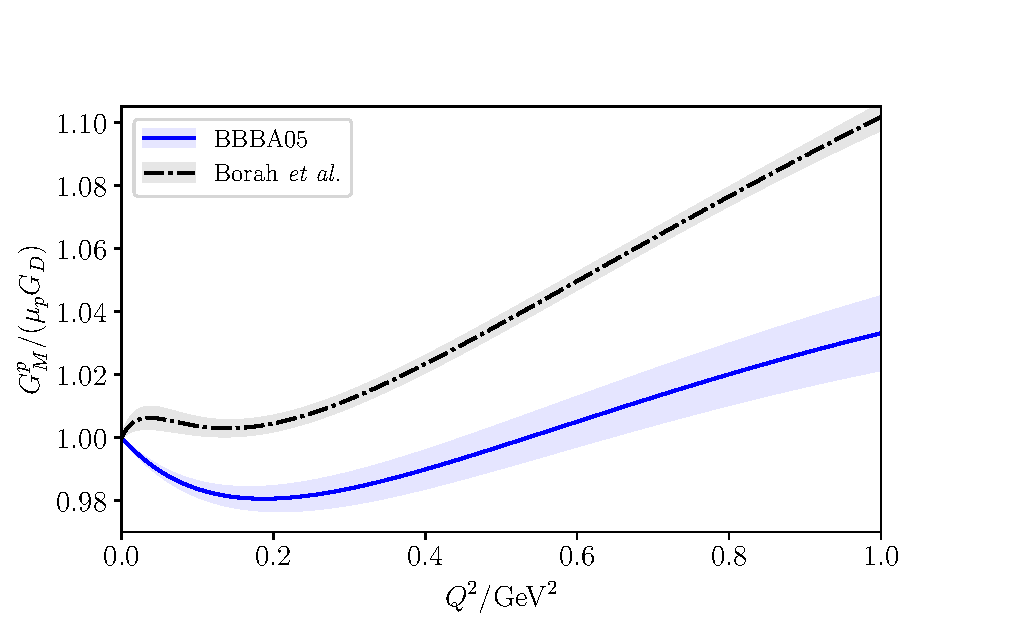
\includegraphics[width=0.5\textwidth]{plots/proton_magnetic-standalone.pdf}
\caption{
 Proton magnetic form factor normalized by a reference dipole ansatz
 with a dipole mass of $0.84~{\rm GeV}$.
 The proton-only fit to a $z$ expansion by Borah {\it et al.}~\cite{Borah:2020gte}
 and the BBBA05 parameterization~\cite{Bradford:2006yz} are shown.
 \label{fig:protonmagneticff}
}
\end{figure}

\begin{figure}[hbt!]
 \centering
 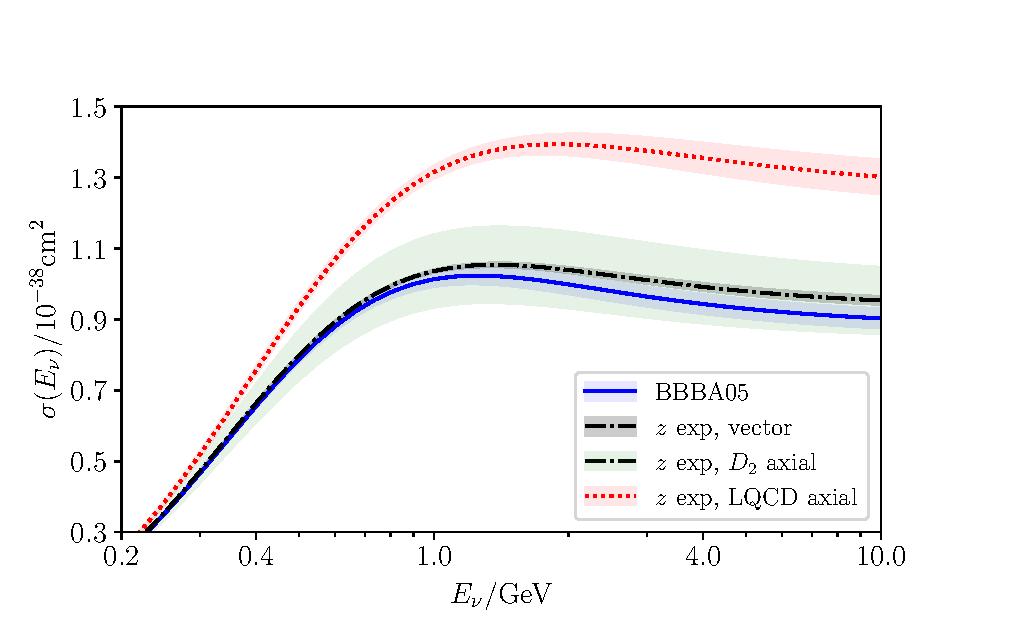
\includegraphics[width=0.5\textwidth]{plots/xsec_comparison-standalone.pdf}
\caption{
 Neutrino cross sections on a free neutron, with their uncertainty bands,
 for various choices of parameterization.
 The curves labeled ``BBBA05'' (blue solid line, Ref.~\cite{Bradford:2006yz})
 and ``$z$ exp, vector'' (black dot-dashed line, Ref.~\cite{Borah:2020gte}) use the
 $z$ expansion axial form factor from Ref.~\cite{Meyer:2016oeg},
 with only the error band from the vector form factors plotted
 to highlight the tension between the parameterizations shown in Fig.~\ref{fig:protonmagneticff}.
 The same form factor parameterizations are used for both ``$z$ exp, vector'' and
 ``$z$ exp, $D_{2}$ axial'' (green dot-dashed line)
 but in the latter case the uncertainty band is taken from the axial form factor
 rather than the vector form factor.
 The red dotted line labeled ``$z$ exp, LQCD axial'' uses the vector form factors
 of Ref.~\cite{Borah:2020gte} with the axial form factor taken from LQCD.
 \label{fig:nucleonxsec}
}
\end{figure}

\begin{description}
\item[first $z$ exp vector form factor] \cite{Ye:2017gyb}
\item[Vector form factor tensions] \cite{Borah:2020gte}
\item[Muonic hydrogen review] \cite{Hill:2017wgb}
\end{description}

\textcolor{red}{[Most focus on axial, but vector is important too]}

